\ProvidesFile{thesis.tex}[2025-01-15 PurdueThesis thesis.tex file]

%  The home page for the PurdueThesis software is
%      https://engineering.purdue.edu/~mark/PurdueThesis/
%
%  Be sure to sign up for the PurdueThesis mailing list at
%      https://engineering.purdue.edu/ECN/mailman/listinfo/purduethesis-list
%  so you learn of new versions of this software.  You must be on that
%  mailing list to receive help with this software.
%
%  This is the template root file for an example thesis (for master's
%  degree) or dissertation (for a Ph.D.).  From now on "thesis" will
%  refer to both of these unless stated otherwise.
%
%  LaTeX systems include auxiliary programs to do bibliographies,
%  indexes, etc.  The latexmk program runs the fewest programs needed
%  to update your thesis.
%
%  On Overleaf (run LaTeX on the web) clicking 'Recompile' will recompile
%  your thesis.
%
%  Use this command on Linux to do all the steps needed to compile your thesis.
%    For Mark Senn:
%      Use
%          latexmk -e '$biber="biber --output-safechars"' -f -g -lualatex --shell-escape thesis
%      to get extra debugging information printed.  Sometimes the `-f -g' can 
%      be deleted to run faster.
%    For everyone else:
%      Use
%          latexmk -e '$biber="biber --output-safechars"' -f -g -lualatex thesis
%      Sometimes the `-f -g' can be deleted to run faster.
%  Here is how that command works:
%      latexmk
%          The latexmk program figures out how to compile
%          your thesis in the quickest way.
%      -e '$biber="biber --output-safechars"'
%          Add the '--output-safechars' option to biber,
%          the command that makes your references.  This
%          command makes accented characters in your references
%          work ok.
%      -f
%          Force latexmk to process your entire thesis, even
%          if it contains errors.
%      -g
%          Force latexmk to process document fully, even under situations
%          where latexmk would normally decide that no changes in the
%          source files have occurred since the previous run.  This  option
%          is  useful, for example, if you change some options and wish to
%          reprocess the files.
%      -lualatex
%          The -lualatex option process your thesis using the LuaLaTeX
%          version of LaTeX.  LuaLaTeX has the Lua programmng language
%          added to make programming LaTeX easier.  You won't need to
%          learn Lua or do any LaTeX programming for your thesis.
%      --shell-escape
%          The --shell-escape option allows you to run external programs
%          from inside your thesis.
%      thesis
%          Process your thesis.tex file.
%
%
%  NOTE TO SELF
%      To count the number of references see
%          https://tex.stackexchange.com/questions/66829/count-number-of-references-using-biblate
%      See set the \labelnumberwidth see page 316 of
%          https://ctan.math.illinois.edu/macros/latex/contrib/biblatex/doc/biblatex.pdf
%      
%
%  PROGRAM                                       BIBLIOGRAPHY    PurdueThesis.cls    thesis.tex   WORKS
%                                                STYLE           RCS rev             RCS rev
%  Mathematics                                   apa             1.249               1.58         yes
%  Mathematics                                   ieee            1.250               1.59         yes
%  Electrical and Computer Engineering           ieee            1.250               1.60         yes
%  Earth, Atmospheric, and Planetary Sciences    apa             1.251               1.61         yes
%  Mathematics                                   apa             1.252               1.62         yes
%  Technology Leadership and Innovation          apa             1.253               1.63         yes
%  Mathematics                                   numeric         ????                ????         ????
%  Earth, Atmospheric, and Planetary Sciences    apa             ????                ????         ????
%

\newcommand{\ZZauthor}{Darin Lin}
\newcommand{\ZZcampus}{West Lafayette}
\newcommand{\ZZdegree}{Master of Science in Aeronautics and Astronautics}
\newcommand{\ZZdocument}{A Thesis}
\newcommand{\ZZgraduation}{December 2025}
\newcommand{\ZZinstitution}{Purdue University}
\newcommand{\ZZprogram}{Aeronautics and Astronautics}

\newcommand{\ZZtitle}{This is the Title}

\newcommand{\ZZshowcolophon}{false}
\newcommand{\ZZshowdiagonalline}{false}
\newcommand{\ZZshowgridlines}{false}
\newcommand{\ZZshowmarginlines}{false}
\newcommand{\ZZshowtimestamp}{false}
\newcommand{\ZZshowtodonotes}{false}

% Mark Senn uses an "optional-debugging-code.tex file" but does not
% distribute it.  The following line won't do anything if you don't
% have an optional-debugging-code.tex file so you can leave it the
% way it is.
\InputIfFileExists{optional-debugging-code.tex}{}{}

% The \includeonly command can be used to only include some
% files that have \include commands below.  This is handy
% to only include some files so your document will LaTeX
% faster or if you're trying to narrow down where an error
% occurs.  You can use
%   \includeonly{ch-introduction}
% to only include ch-introduction.tex, or
%   \includeonly{ch-introduction,ap-about-appendices}
% to include ch-introduction.tex and ap-about-appendices.tex.
% More files can be added---just put ',' between the names.
% Comment out the following line before submitting the
% final copy of your thesis.
%\includeonly{ch-introduction,ap-about-appendices}


\documentclass{PurdueThesis}

\newcommand{\ZZatinformation}{}

\graphicspath{{graphics/}}
\makeatletter
  \def\input@path{{misc}{packages}}
\makeatother

\ConfigureBibliography

% For \bm.
% The bm package was last updated on 2022-01-05.
\usepackage{bm}


% Define
%    \VerbatimInput[options]{filename}
%    \begin{VerbatimOut}{filename} ... \end{VerbatimOut}.
\usepackage{fancyvrb}
  % So '|verbatim|' will print 'verbatim' in a typewriter font.
  % If you don't want this, put a '%' before the next line.
  \DefineShortVerb{\|}

\usepackage{listings}

% Include XMP data in a PDF document.
% See
%   http://mirrors.ibiblio.org/CTAN/macros/latex/contrib/hyperxmp/hyperxmp.pdf
% for more information including all the possible fields that can be set.
\usepackage{hyperxmp}
  \hypersetup{
    pdfauthor    = {Mark Senn},
    pdfcopyright = {Copyright \copyright\ 2024 by Mark Senn.  All rights reserved.},
    % Use `yyyy-mm' format where `yyyy' is year and `mm' is month.
    pdfdate      = {2025-05},
    pdfkeywords  = {LaTeX; Purdue University; PurdueThesis},
    pdflang      = {en},
    pdfpublisher = {Purdue University},
    pdfsubject   = {%
                     PurdueThesis is a LaTeX document class used for
                     master's bypass reports,
                     master's theses,
                     PhD dissertations,
                     and PhD preliminary reports.
                     This template demonstrates how to use PurdueThesis.%
                   },
    pdftitle     = {This is the Title},
  }

\usepackage{mathtools}
\usepackage{amsfonts}
\usepackage{multicol}
\usepackage{pa-logos}
\def\pa{\rotatebox[origin=c]{14}{\partial}}
\def\Fourier{\mathcal{F}}
\def\Laplace{\mathcal{L}}
\usepackage{pa-repeat}
\usepackage{placeins}

% Needed for chapter "Graphics", section "TikZ and PGF".
\usepackage{tikz}
  % Needed to customize arrows.
  \usetikzlibrary{arrows.meta}
  % For electrical diagrams.
  % Uses the TikZ package.
  % The circuitikz name is short for "circuit TikZ".
  \usepackage{circuitikz}
  %
  \usepackage{menukeys}
  %
  % Needed for 3D TikZ stuff.
  \usetikzlibrary{3d}
  %
  % Needed for pa-typographic-conventions package.
  \usetikzlibrary{calc,shadows,shapes.misc,shapes.symbols}
  %
  % Needed for putting text along a path.
  \usetikzlibrary{decorations.text}
  %
  % Draw TikZ decorations.
  % Needed for at least the Kalman filter system model graphic.
  \usetikzlibrary{decorations.pathmorphing} % noisy shapes
  %
  % Fit shapes to coordinates.
  % Needed for at least the Kalman filter system model graphic.
  \usetikzlibrary{fit}
  %
  % Draw the background after the foreground.
  \usetikzlibrary{backgrounds}	% drawing the background after the foreground

% The vertical space between a table heading and the table contents
% in a tabular environment.
\newcommand{\tabularspace}{\noalign{\vspace*{2pt}}}

% For \sfrac, used to do slanted fractions, similar to, e.g., 1/2,
% but 1 is small and high and 2 is small and low.
\usepackage{xfrac}


% Define \I.
% \I1 does \indent once, \I2 does \indent twice, etc.
\newcommand{\I}[1]{\MyRepeat{\indent}{#1}}

% Define \MyI.
% Typeset my input.
\long\def\MyI#1%
  {%
    {%
      \fontsize{8}{10}\tt
      \VerbatimInput
        [
          firstnumber = 1,
          numbers     = left,
          xleftmargin = 0.33in,
        ]%
        {#1}
    }%
  }

% Define \MyIO.
% Typeset my input and output.
% The input will all be on the same page.
% The output may be split over multiple pages.
\newcommand{\MyIO}
  {%
    \input{z.out}

    {%
      \fontsize{8}{10}\tt
      \VerbatimInput
        [
          firstnumber = 1,
          numbers     = left,
          xleftmargin = 0.33in,
        ]
        {z.out}
    }
    \FloatBarrier
  }

% Define \NL (newline) so LaTeX goes to the next output line.
% Just doing \\ complains
%     ! LaTeX Error: There's no line here to end.
% \mbox{} is an empty math box.
\newcommand{\NL}{\mbox{}\\}

% In this document I use in-line tables a lot.
% These are tables that are put in the document
% where I want them to appear and they don't
% use \begin{table} ... \end{table}
\newenvironment{inlinetable}
  {%
    \begingroup
      \singlespace
      \mbox{}\\[-9pt]%
      \noindent
      \hspace*{2\parindent}%
      \ignorespaces
  }
  {%
      \mbox{}\\
    \endgroup
  }

\listfiles
\usepackage{pa-typographic-conventions}

% New definitions and math commands here
\DeclareMathOperator*{\argmax}{arg\,max}
\DeclareMathOperator*{\argmin}{arg\,min}

\begin{document}

\makeatletter
\renewcommand{\ZZAppendixName}{APPENDIX}
%%%% \renewcommand{\chaptername}{CHAPTER}
\def\@@makechapterhead#1{\uppercase{\@chapapp~\thechapter. #1}}

\setcounter{tocdepth}{3}

\maketitle

\ProvidesFile{ch-front.tex}[2024-09-12 front matter chapter]
%
%  This is the ``front matter'' for the thesis.
%
%  REFERENCES
%
%    TCMOS17
%      The Chicago Manual of Style Online, 17th edition.
%      https://www.chicagomanualofstyle.org/home.html
%      retrieved on 2020-02-29
%
%    TEMPL
%      Thesis and Disertation Office Templates.
%      https://www.purdue.edu/gradschool/research/thesis/templates.html
%      retrieved on 2020-02-29
%
%    WNNCD
%    Webster's Ninth New Collegiate Dictionary.
%

%
%   Only Purdue University uses this page
%
%   Comment out \begin{statement} through \end{statement}
%   if you are not at Purdue University.
%
% Statement of Thesis/Dissertation Approval Page
% This page is REQUIRED.  The page should be numbered "2"
% and should NOT be listed in your TABLE OF CONTENTS.
\begin{statement}
  % Delete or add \entry commands as needed for all committe members.
  \entry{Dr.~Kenshiro Oguri, Chair}{School of Aeronautics and Astronautics}
  \entry{Dr.~Inseok Hwang}{School of Aeronautics and Astronautics}
  \entry{Dr.~Keith LeGrand}{School of Aeronautics and Astronautics}
  % There should be one \approvedby command containing the
  % "FORM 9 THESIS FORM HEAD NAME HERE" (from TEMPL, retrieved on 2020-03-01).
  \approvedby{Dr.~Buck Doe}
\end{statement}

% Dedication page is optional.
% A name and often a message in tribute to a person or cause.
% References: WEB9 332.
\begin{dedication}
  To graduate students
\end{dedication}

% Acknowledgements page is optional but most theses include
% a brief statement of appreciation or recognition of special
% assistance.
\begin{acknowledgments}
  Purdue University's Engineering Computer Network
  (now part of Purdue IT)
  and Graduate School helped fund \PurdueThesisLogo\ development.
\end{acknowledgments}

% The preface is optional.
% References: TCMOS17 1.49, WEB9 927.
\begin{preface}
  This is the preface.
\end{preface}

% The Table of Contents is required.
% The Table of Contents will be automatically created for you
% using information you supply in
%     \chapter
%     \section
%     \subsection
%     \subsubsection
%     commands.
\pdfbookmark{TABLE OF CONTENTS}{Contents}
\tableofcontents

% If your thesis has tables, a list of tables is required.
% The List of Tables will be automatically created for you using
% information you supply in
%     \begin{table} ... \end{table}
% environments.
\listoftables

% If your thesis has figures, a list of figures is required.
% The List of Figures will be automatically created for you using
% information you supply in
%     \begin{figure} ... \end{figure}
% environments.
\listoffigures

% If your thesis has listings, a list of listings is required.
% The List of Listings will be automatically created for you using
% information you supply in
%     \begin{ZZlisting} ... \end{ZZlisting}
% environments.
\ZZlistoflistings

% List of Symbols is optional.
\begin{symbols}
  \(m\)& mass\cr
  \(v\)& velocity\cr
\end{symbols}

% List of Abbreviations is optional.
\begin{abbreviations}
  abbr& abbreviation\cr
  bcf& billion cubic feet\cr
  BMOC& big man on campus\cr
\end{abbreviations}

\begin{abstract}
  Tracking maneuvering cislunar spacecraft is a difficult task due to the highly nonlinear dynamical environment, great distances, and frequent observation gaps. If optimal control is assumed, it is possible to predict the future control of a spacecraft given observations of the start of a maneuver. This idea is applied to construct an optimal control interacting multiple model estimator (OCIMM) by including the costate as an estimation variable. The OCIMM can significantly reduce the mean absolute estimation error compared to a traditional IMM during observation gaps and periods of rapidly changing control through its ability to predict the future control. 
\end{abstract}


\ProvidesFile{ch-important.tex}[2024-07-12 important chapter]

\chapter{IMPORTANT---READ THIS FIRST}

Be sure to sign up for the
\href{https://engineering.purdue.edu/ECN/mailman/listinfo/purduethesis-list}{\PurdueThesisLogo\ mailing list}%
\cite{PurdueThesis-mailing-list}
to learn of important changes to
or get help with \PurdueThesisLogo.

I suggest you do not make any changes
to the |PurdueThesis.cls| file.
Put any changes in the |thesis.tex| file if you can.
That way you will not need to add your customizations
when a new version of |PurdueThesis.cls| is released.


\ProvidesFile{ch-introduction.tex}

\chapter{INTRODUCTION}

International interest in cislunar space has increased significantly in the recent decade \cite{nelson2024moon}. Space domain awareness (SDA) will be critical for the future sustainable development of cislunar space. Compared to SDA near Earth, cislunar SDA faces significant challenges due to highly nonlinear cislunar dynamics, extreme distances, and frequent observation gaps. To add to this complexity, active cislunar spacecraft have the ability to maneuver, which in combintation with the chaotic cislunar dynamics further compounds the extreme nonlinearity of the tracking problem. Additionally, low-thrust propulsion has become an increasingly popular choice for spacecraft because of its high specific impulse, allowing for longer mission durations and smaller fuel fractions. Thus, tracking low-thrust maneuvering spacecraft in cislunar space is a problem of interest. 

Significant research effort has been dedicated to the general maneuvering target tracking problem. Bar-Shalom et al. presents several sequential algorithms to account for the discrete nature of maneuvering objects, most notably the interacting multiple model estimator \cite{bar1989tracking} (IMM) and the variable state dimension estimator \cite{bar2007variable} (VSD). Goff et al. implements a combination of these algorithms specifically for tracking low-thrust maneuvering spacecraft in geocentric orbits \cite{goff2015orbit}. Wetterer et al. utilizes an IMM to track impulsively maneuvering spacecraft in cislunar space \cite{wetterer2022cislunar}.

Other research efforts have been dedicated to manage the nonlinearity of the problem. DeMars et al. model the true uncertainty distribution as a mixture of Gaussian distributions, where the number of Gaussian kernels is adaptively increased and decreased in areas of higher and lower nonlinearity, respectively, where nonlinearity is detected via entropy \cite{demars2013entropy}. They then apply this algorithm to accurately model the uncertainty distribution of a spacecraft in geocentric orbit. Vishwjeet and Singla similarly apply a Gaussian mixture-based approach, instead detecting nonlinearity using the Kolmogorov equation error \cite{vishwajet2018adaptive}. 

% \begin{figure}
%     \centering
%     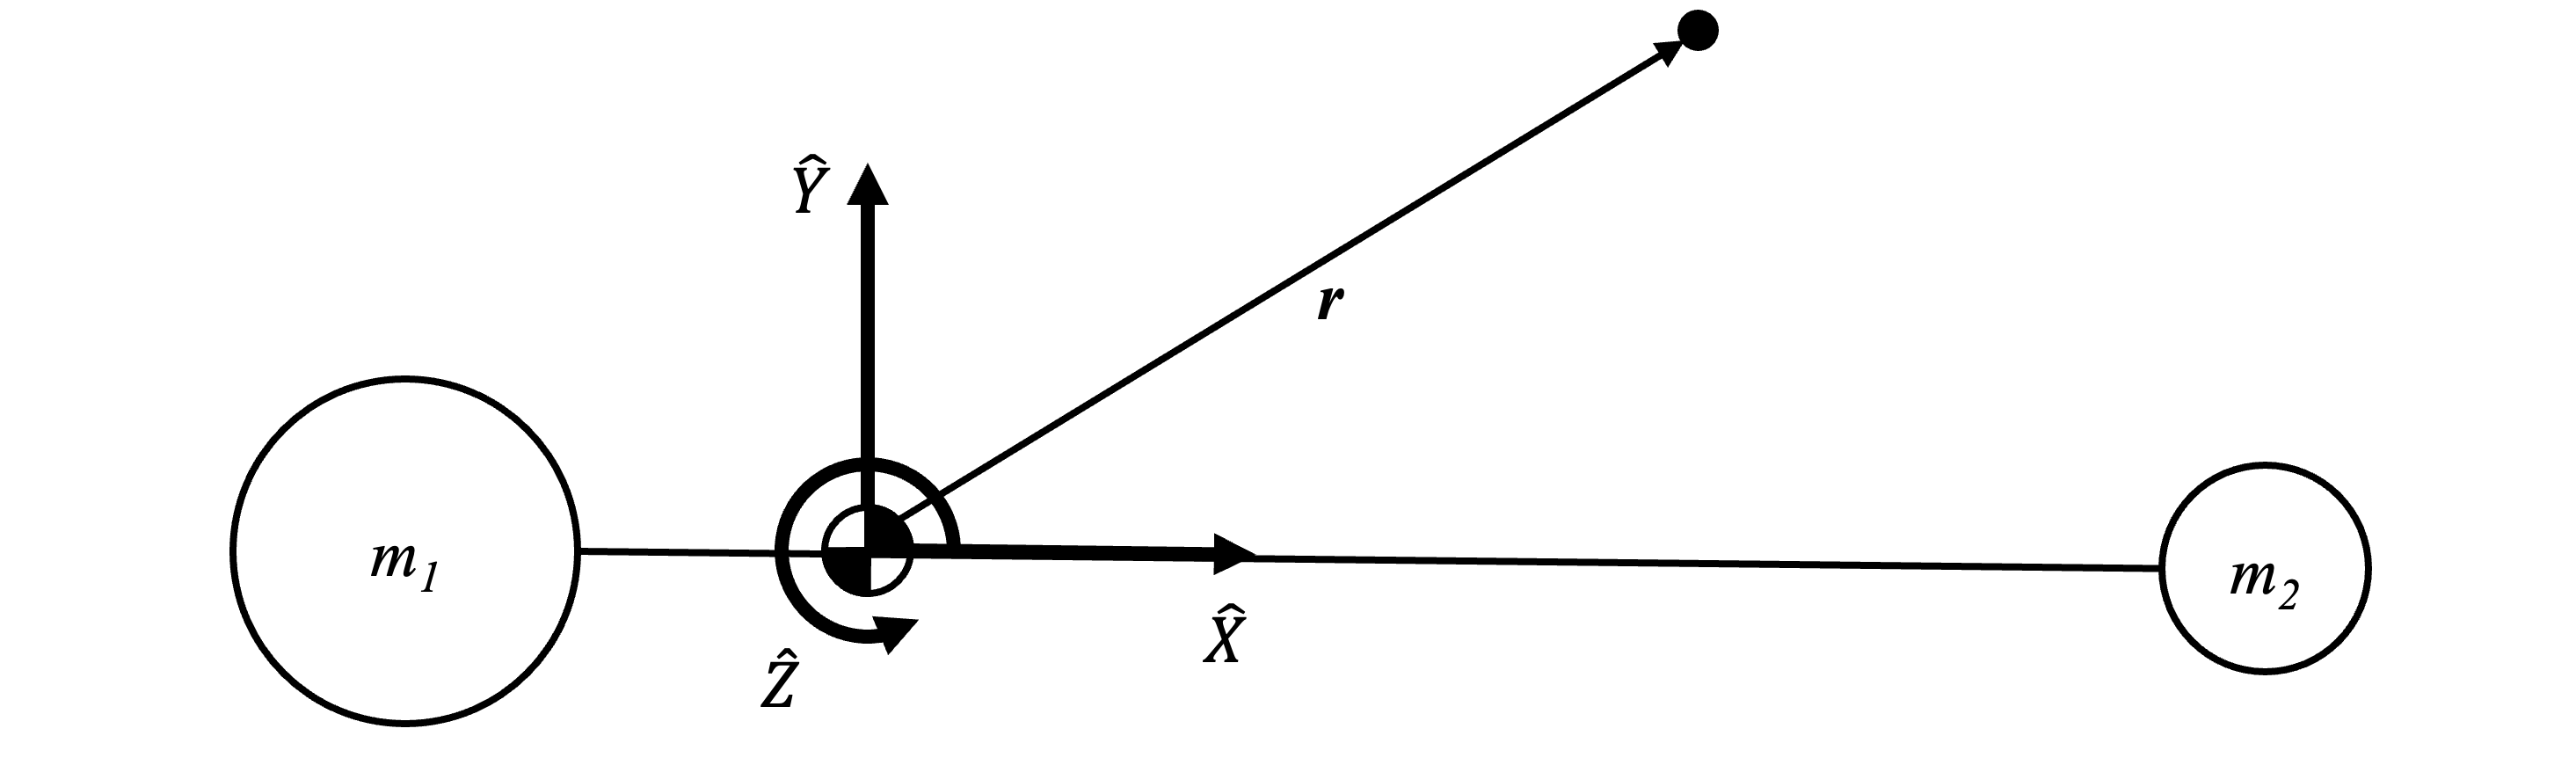
\includegraphics[width=1\linewidth]{Figures/CR3BP.png}
%     \caption{Circular-Restricted Three-Body Problem Coordinate Frame}
%     \label{fig:CR3BP}
% \end{figure}

Iannamorelli and LeGrand combine the adaptive Gaussian mixture and multiple model estimation approaches to simultaneously combat the extreme nonlinearity of cislunar dynamics and account for the maneuvers of a spacecraft \cite{iannamorelli2025adaptive}. Their adaptive Gaussian mixture interacting multiple model estimator (AGMIMM) models maneuvers as zero-mean, Gaussian process noise, so if properly tuned to capture all possible spacecraft maneuvers, the AGMIMM is able to accurately determine where the spacecraft \textit{could} be. However, it is reasonable to assume that the maneuvers of the target spacecraft will be optimal, in which case modeling maneuvers as zero-mean process noise would be overly-conservative. If instead some optimal control law is assumed, given observations of the beginning of a maneuver, it is possible to predict where the spacecraft \textit{should} be at some future time with less uncertainty than by modeling maneuvers as zero-mean process noise. As cislunar SDA becomes more complex with more cislunar spacecraft, decreasing this uncertainty will be critical for correlating tracks of multiple maneuvering targets and allocating limited observational resources.

The concept of using optimal control to improve tracking is explored by Holzinger et al., resulting in the development of the control-distance metric \cite{holzinger2012object}. The control-distance metric characterizes the amount of control effort required to connect two spacecraft states assuming some optimal control, thus allowing the correlation of tracks which are separated by smaller control distances. Lubey and Scheeres apply this framework to develop a sequential estimator, resulting in the Optimal Control-Based Estimator (OCBE) \cite{lubey2013optimal}. The OCBE models any deviation in the state dynamics as an optimal control, which allows both control inputs and mismodeled dynamics to be reconstructed from these deviations. The OCBE is applied by Greaves and Scheeres to the cislunar tracking problem for maneuver detection and reconstruction \cite{greaves2021observation}. These approaches, however, are for the posterior reconstruction and detection of maneuvers rather than for the prior prediction of maneuvers. 

The main contribution of this paper is the implementation of an assumed optimal control policy directly into the dynamics of an adaptive multiple-model estimator. An IMM with two modes is utilized, where the non-maneuvering (coasting) mode assumes ballistic dynamics, and the maneuvering (thrusting) mode assumes a minimum-time optimal control policy. The dynamics of the minimum-time optimal control policy are obtained using Pontryagin's minimum principle \cite{pontryagin1962}. This optimal control IMM (OCIMM) is used to track a cislunar spacecraft performing a low-thrust transfer between two periodic cislunar orbits under a fuel-optimal control policy, whose thrusting arcs follow the same dynamics of a time-optimal policy. The OCIMM is shown to be able to accurately predict the future control inputs of the target spacecraft, even during observation gaps and periods of rapidly changing control. This results in superior estimation performance compared to a traditional IMM. 


\ProvidesFile{ch-theory.tex}

\chapter{THEORY}

\section{Circular-Restricted Three-Body Problem (CR3BP) with Control}

To model the motion of a maneuvering spacecraft in cislunar space, we utilize the circular restricted three-body problem dynamics model with low-thrust control modeled as an affine acceleration. This model assumes circular motion of two massive primary bodies around their barycenter. A third massless body is then subject to the gravities of the other two massive bodies. This third body represents the spacecraft of interest, and its state $\bm{\xi} = [\bm{r}^\top, \bm{v}^\top]^\top$ consists of a three-dimensional position and velocity, $\bm{r} = [x, y, z]^\top$ and $\bm{v} = [v_x, v_y, v_z]^\top$, respectively. The control is a three-dimensional additive acceleration $\bm{u} = [u_x, u_y, u_z]^\top$. To define the coordinate frame, the origin is fixed at the barycenter, the X-axis is aligned with the line between the two massive bodies, the Z-axis is aligned with the angular velocity vector, and the Y-axis completes the X-Y-Z right-handed coordinate frame. The CR3BP coordinate frame is illustrated in Figure \ref{fig:CR3BP}. 

The units of the system are normalized such that the unit length is the distance between the two massive bodies, and the unit time is the inverse of the angular velocity of the two massive bodies. The motion of the massless body is then described by a system of nonlinear differential equations given by 
\begin{align}
\begin{aligned}
    \dot{\bm{\xi}} &= \bm{g}(\bm{\xi}) + B\bm{u}= \begin{bmatrix}
        v_x \\
        v_y \\
        v_z \\
        -\frac{(1 - \mu)(x + \mu)}{d^2} - \frac{\mu(x + \mu - 1)}{r^2} + 2v_y + x\\
        -\frac{(1 - \mu)y}{d^2} - \frac{\mu y}{r^2} - 2v_x + y\\
        -\frac{(1 - \mu)z}{d^2} - \frac{\mu z}{r^2}
    \end{bmatrix} + \begin{bmatrix}
        0_{3 \times 3} \\
        I_3
    \end{bmatrix} \begin{bmatrix}
        u_x \\
        u_y \\
        u_z
    \end{bmatrix} \\
    d &= \sqrt{(x+\mu)^2 + y^2 + z^2}, \quad r = \sqrt{(x + \mu - 1)^2 + y^2 + z^2} \label{eq:CR3BP-dynamics}
\end{aligned}
\end{align}
\noindent where $\mu = m_2/(m_1 + m_2)$ is the ratio of the second body's mass to the total mass of the system \cite{zimovan2017characteristics}.

\section{Periodic Orbits in the CR3BP}

% \begin{figure}
%     \centering
%     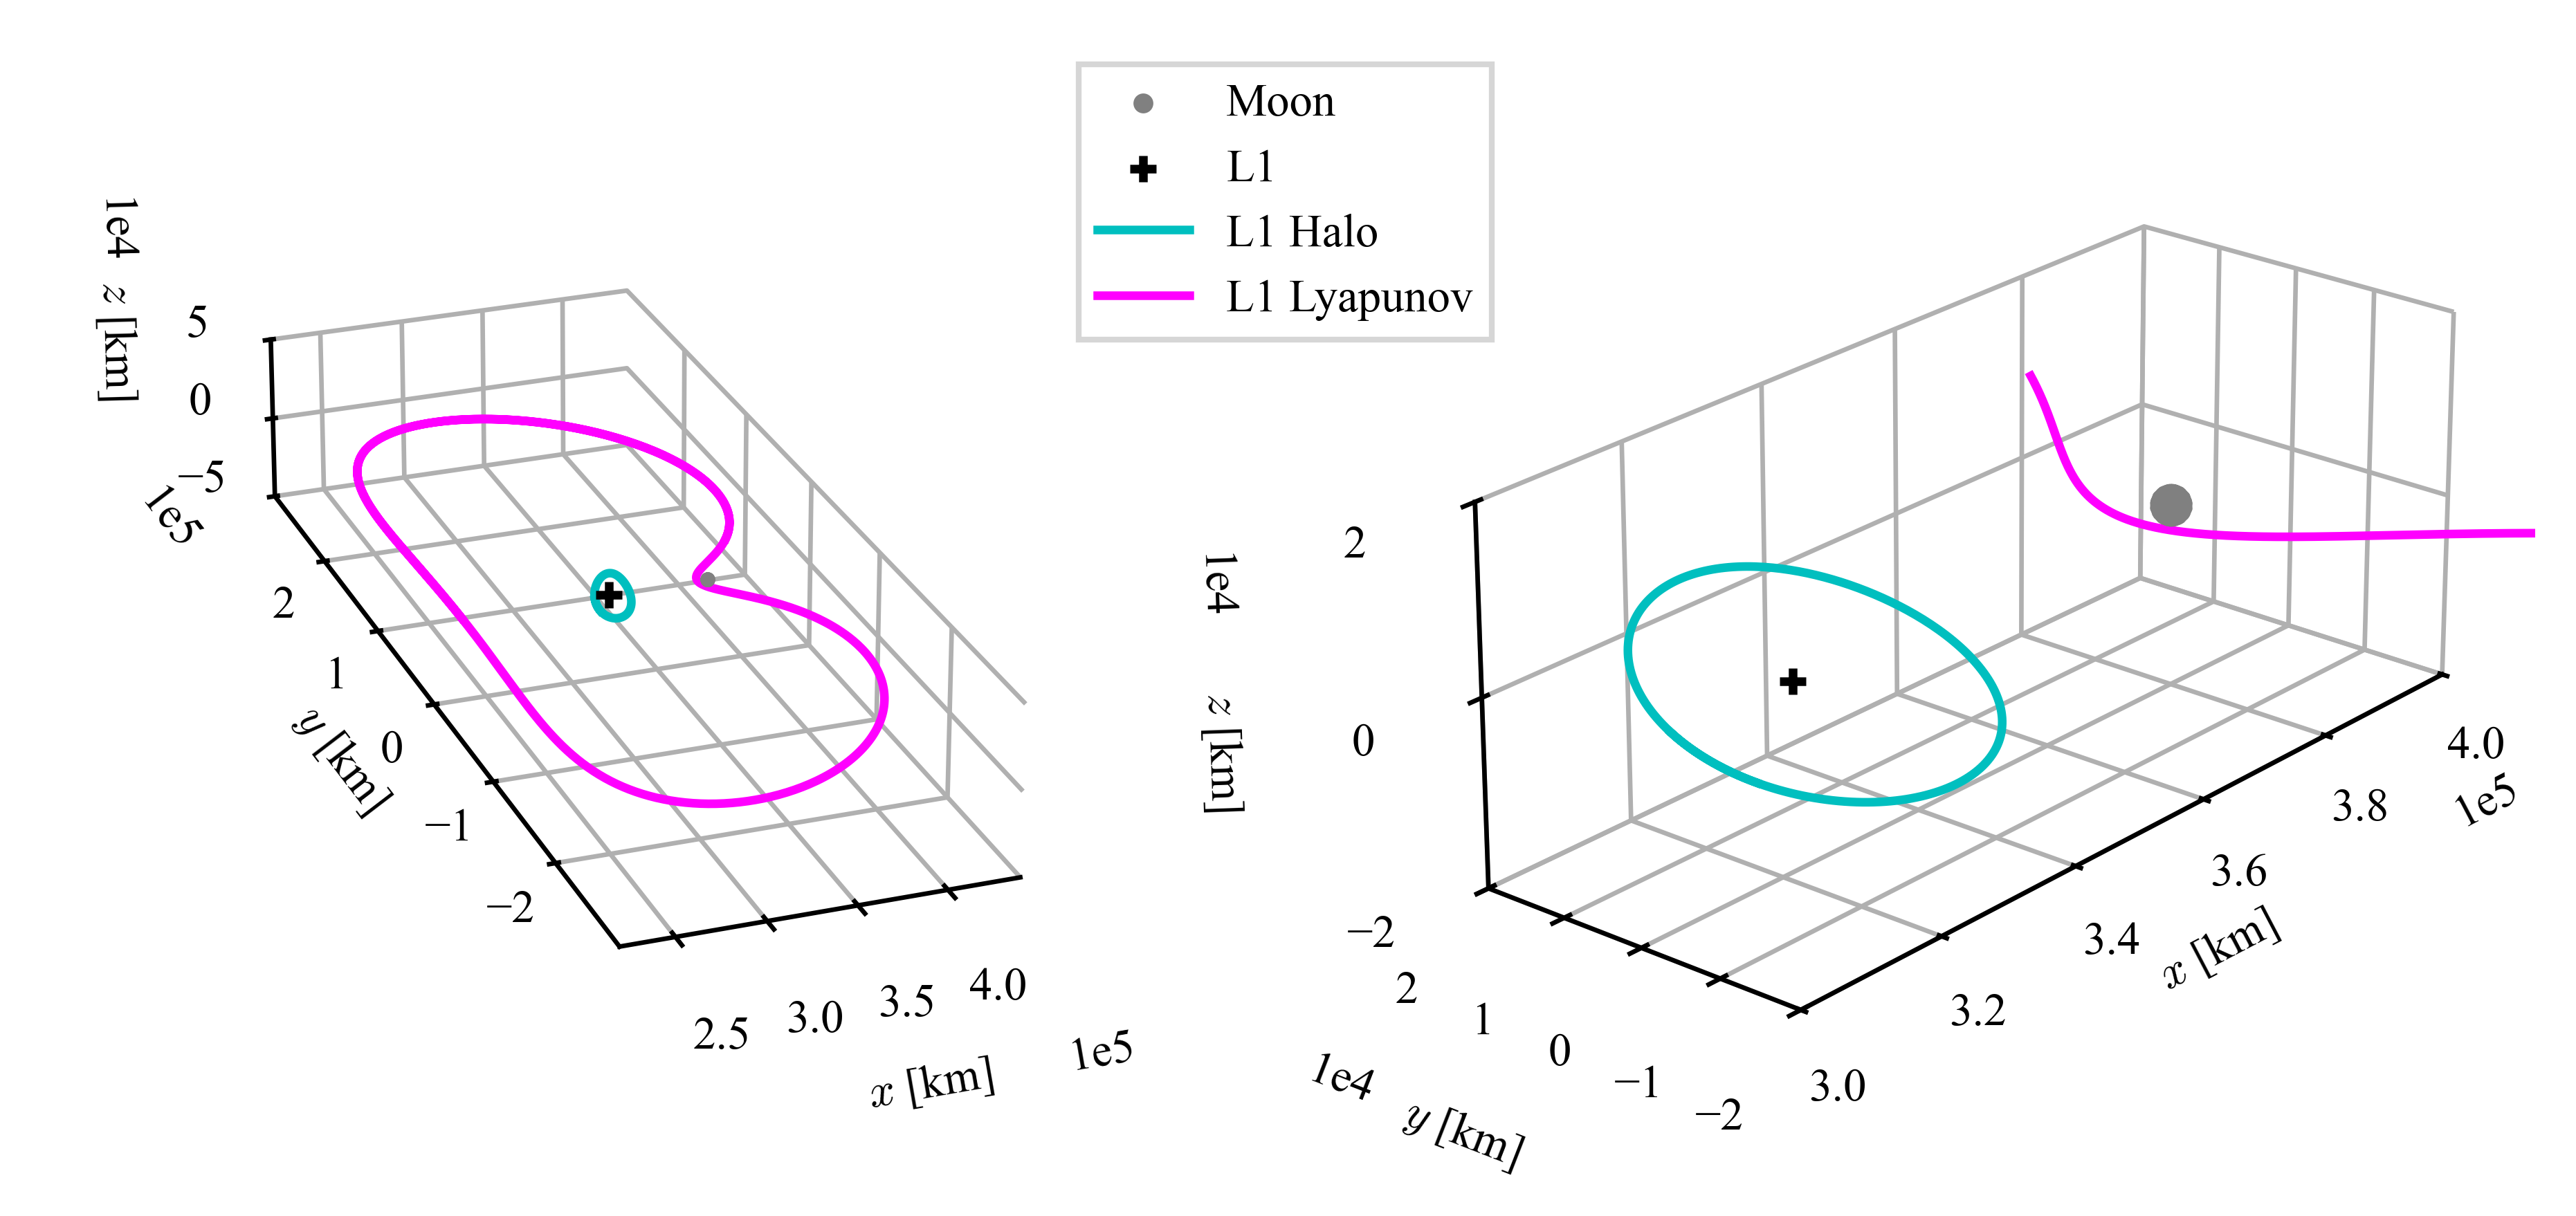
\includegraphics[width=0.85\linewidth]{Figures/orbits.png}
%     \caption{Representative L1 Lyapunov and L1 Halo Periodic Orbits}
%     \label{fig:orbits}
% \end{figure}

It is desirable to obtain periodic solutions $\bm{\gamma}$ to the CR3BP dynamics (Eq. \ref{eq:CR3BP-dynamics}), such that
\begin{align}
    \bm{\gamma}(t + T) = \bm{\gamma}(t)
\end{align}
\noindent where $T$ is the period of the solution. These periodic orbits enable geometries impossible when only considering a single body's gravity. However, the dynamics of the CR3BP (Eq. \ref{eq:CR3BP-dynamics}) have no analytical closed-form solution, so these orbits are typically obtained using numerical methods.

Once a periodic solution has been obtained, continuation strategies can be employed to obtain a family of similar solutions \cite{williams2024dynamics}. The orbits of interest in this paper are those belonging to the L1 Lyapunov and L1 Halo families. These families are associated with the L1 Lagrange point, with the L1 Lyapunov family lying in the xy-plane and the L1 Halo family being three dimensional. These solutions are unstable, increasing the difficulty of the tracking problem, as small estimation errors caused by perturbations or maneuvers quickly expand during periods without observations. The representative orbits of interest are plotted in Figure \ref{fig:orbits}.

\section{Extended Kalman Filter (EKF)}

The ubiquitous Extended Kalman Filter (EKF) is an recursive estimation algorithm for systems with nonlinear dynamics/measurements \cite{smith1962application}. One iteration of the continuous-discrete EKF consists of two steps: a continuous time update and a discrete measurement update.

\begin{enumerate}
    \item Time Update
    
    The time update propagates the posterior estimate ${}^+\hat{\bm{x}}_{k-1}$ and estimation error covariance ${}^+P_{k-1}$ at the time of the previous measurement $t_{k-1}$ to the time of the current measurement $t_k$. The state is propagated with the nonlinear dynamics equation $\dot{\bm{x}} = \bm{f}(\bm{x})$, and the covariance is propagated with the state transition matrix $\Phi(t_k, t_{k-1})$ and process noise covariance $Q_{k-1}$, yielding the prior estimate and covariance at the current time, ${}^-\bm{\hat{x}}_k$ and ${}^-P_k$:
    \begin{align}
        {}^-\hat{\bm{x}}_k &= \int_{t_{k-1}}^{t_k} \bm{f}(\bm{\hat{x}}(t)) dt, & \hat{\bm{x}}(t_{k-1}) = {}^+\hat{\bm{x}}_{k-1} \label{nonlinear estimate propagation (first EKF equation)} \\
        {}^-P_k &= \Phi(t_k, t_{k-1}) {}^+P_{k-1} \Phi^\top(t_k, t_{k-1}) + Q_{k-1}\\
        \Phi(t_k, t_{k-1}) &= \int_{t_{k-1}}^{t_k} F(\hat{\bm{x}}(\tau))\Phi(\tau, t_{k-1}) d\tau, & \Phi(t_{k-1}, t_{k-1}) = I_{n\times n} \label{eq:STM-propagation}
    \end{align}
    Additionally, the nonlinear measurement equation $\bm{z} = \bm{h}(\bm{x})$ is applied to the prior estimate ${}^-\hat{\bm{x}}_k$ to obtain the predicted measurement, $\bm{\hat{z}}_k$.
    \begin{align}
        \bm{\hat{z}}_k = \bm{h}_k(\bm{\hat{x}}_k^-) \label{eq:predicted measurement}
    \end{align}

    \item Measurement Update
    
    After the time update, ${}^-\bm{\hat{x}}_k$ and ${}^-P_k$ are updated with the new measurement $\bm{z}_k = \bm{h}_k(\bm{x}_k) + \bm{w}_k$ to obtain the posterior estimate and covariance, ${}^-\bm{x}_k$ and ${}^+P_k$. Mathematically,
    \begin{align}
        ^+\bm{\hat{x}}_k &= K_k (\bm{z}_k - \bm{\hat{z}}_k) \label{eq:posterior-estimate-update}\\
        ^+P_k &= {}^-P_k - C_k K_k^\top - K_k C_k ^\top + K_k W_k K_k^\top \\
        K_k &= C_k W_k^{-1} \\
        C_k &= {}^-P_k H_k^\top({}^-\bm{\hat{x}}_k) \\
        W_k &= H_k({}^-\bm{\hat{x}}_k) {}^-P_k H_k^\top({}^-\bm{\hat{x}}_k) + R_k \label{eq:innovations covariance (last EKF eq)}
    \end{align}
    \noindent where $K_k$ is the Kalman gain matrix, $C_k$ is the cross covariance matrix, $W_k$ is the innovations covariance matrix, $H_k({}^-\bm{\hat{x}}_k) = \partial \bm{h}({}^-\hat{\bm{x}}_k)/\partial\bm{x}$ is the measurement Jacobian, and $R_k = \mathcal{E}[\bm{w}_k\bm{w}_k^\top]$ is the measurement noise covariance.

\end{enumerate}

At the completion of the measurement update, one iteration of the EKF is completed, and the next iteration begins after setting $ t_k \rightarrow t_{k-1}$. 

\section{Interacting Multiple Model (IMM) Estimator}

The interacting multiple model (IMM) estimator is well-suited for tracking maneuvering targets because of its ability to incorporate multiple dynamics models into a single filter \cite{blom1988interacting,bar1989tracking,genovese2001interacting}. These different dynamics models can capture the discrete ``modes" of a maneuvering target which yields a more accurate estimate. 

Mathematically, the IMM assumes that the target's mode $\tau_k$ at time $t_k$ is one of $s$ discrete modes in the set of all modes $M = \{1, \cdots, s\}$, such that $\tau_k \in M $. Each mode $j \in M$ is associated with a dynamics model $\dot{\bm{x}} = \bm{f}^{(j)}(\bm{x})$, process noise covariance $Q^{(j)}$, posterior state estimate ${}^+\hat{\bm{x}}_k^{(j)}$, posterior estimate error covariance ${}^+P_k^{(j)}$, and mode probability $\mu^{(j)}_k = \mathbb{P}\{\tau_k = j\}$. The time evolution of these modes are modeled as a discrete-time Markov chain with associated row-stochastic transition matrix $\Pi \in \mathbb{R}^{s \times s}$, where element $\Pi_{i, j} = \mathbb{P}\{\tau_k=j \mid \tau_{k-1} = i\}$.

One iteration of the IMM consists of three steps: probabilistic mixing, mode-dependent filtering, and mode probability update.

\begin{enumerate}
    \item Probabilistic Mixing

    The posterior state estimates ${}^+\hat{\bm{x}}_{k-1}^{(j)}$ and covariances ${}^+P_{k-1}^{(j)}$ are probabilistically combined to create mode-matched initial conditions for the mode-dependent filtering in the following step. The mode-matched estimate and covariance for each mode $j$ is denoted as ${}^{+}\hat{\bm{x}}_{k-1}^{0j}$ and ${}^+P_{k-1}^{0j}$, respectively, and are obtained with
    \begin{align}
        {}^+\hat{\bm{x}}_{k-1}^{0j} &= \sum_{i=1}^r {}^+\hat{\bm{x}}_{k-1}^{(i)} \mu_{k-1}^{i \mid j} \label{eq:mixed-initial-mean}\\
        {}^+P_{k-1}^{0j} &= \sum_{i=1}^r  \mu_{k-1}^{i \mid j} [{}^+P_{k-1}^{(i)} + ({}^+\bm{\hat{x}}_{k-1}^{(i)} - {}^+\bm{\hat{x}}_{k-1}^{0j})({}^+\bm{\hat{x}}_{k-1}^{(i)} - {}^+\bm{\hat{x}}_{k-1}^{0j})^\top ] \label{eq:mixed-initial-covariance}
    \end{align}
    \noindent where $\mu_k^{i \mid j}$ is the mixing probability, which captures how much of mode $i$'s posterior estimate should be mixed into mode $j$'s initial conditions. The mixing probabilities $\mu_k^{i \mid j}$ are computed as
    \begin{align}
        \mu_{k-1}^{i \mid j} &= \frac{1}{\bar{c}_{k-1}^{(j)}} \Pi_{i,j} \mu_{k-1}^{(i)} \\
        \bar{c}_{k-1}^{(j)} &= \sum_{i=1}^r \Pi_{i,j} \mu_{k-1}^{(i)} \label{mixing probability constant}
    \end{align}
    \noindent where $\bar{c}_{k-1}^{(j)}$ is a normalization constant such that $\sum_{i=1}^r \mu_{k-1}^{i \mid j} = 1$.
    
    \item Mode-Dependent Filtering

    After constructing the mode-matched initial conditions, an iteration of the EKF is performed for each mode $j \in M$ with Eqs. \ref{nonlinear estimate propagation (first EKF equation)}-\ref{eq:innovations covariance (last EKF eq)}, each with its own mode-matched initial conditions ${}^+\bm{\hat{x}}_{k-1}^{0j}$ and ${}^+P_{k-1}^{0j}$, dynamics equation $\bm{f}^{(j)}(\bm{x})$, and process noise covariance $Q^{(j)}$. This yields the posterior estimates and covariances for each mode ${}^+\hat{\bm{x}}_k^{(j)}$ and ${}^+P_k^{(j)}$.

    \item Mode Probability Update

    In addition to obtaining ${}^+\hat{\bm{x}}_k^{(j)}$ and ${}^+P_k^{(j)}$, the mode probabilities are updated according to the innovations likelihoods $\Lambda_k^{(j)}$ given by
    \begin{align}
        \Lambda_k^{(j)} = \dfrac{1}{\sqrt{\mid 2\pi W_k^{(j)} \mid}} \exp[-\frac{1}{2} (\bm{z}_k - \bm{\hat{z}}_k^{(j)})^\top (W_k^{(j)})^{-1} (\bm{z}_k - \bm{\hat{z}}_k^{(j)})] \label{eq:innovations-likelihoods}
    \end{align}
    where $W_k^{(j)}$ is mode $j$'s innovations covariance defined in Eq. \ref{eq:innovations covariance (last EKF eq)}, and $\hat{\bm{z}}_k^{(j)}$ is mode $j$'s predicted measurement defined in Eq. \ref{eq:predicted measurement}. The mode probability update is 
    \begin{align}
    \mu_k^{(j)} & = \frac{1}{c_k} \Lambda_k^{(j)} \bar{c}_{k-1}^{(j)} \label{eq:mode-probability-update} \\
    c_k &= \sum_{i=1}^r \Lambda_k^{(i)} \bar{c}_{k-1}^{(i)} 
    \end{align}
    where $\bar{c}_{k-1}^{(j)}$ is defined in Eq. \ref{mixing probability constant} and $c_k$ is a normalization constant such that $\sum_{j=1}^r \mu_k^{(j)} = 1$. The computation of the mode probabilities concludes a single iteration of the IMM, and the next iteration begins after setting $t_k \rightarrow t_{k-1}$.

    \item Output

    To obtain a single output value for the posterior estimate ${}^+\hat{\bm{x}}_k$ and posterior covariance ${}^+P_k $, the various posterior estimates ${}^+\hat{\bm{x}}_k^{(j)}$ and covariances ${}^+P_k^{(j)}$ are combined using their mode probabilities $\mu_k^{(j)}$:
    \begin{align}
        {}^+\bm{\hat{x}}_k &= \sum_{j=1}^r \mu_k^{(j)} {}^+\bm{\hat{x}}_k^{(j)}  \\
        {}^+P_k &= \sum_{j=1}^r \mu_k^j [{}^+P_k^{(j)} + ({}^+\bm{\hat{x}}_k^{(j)} - {}^+\bm{\hat{x}}_k)({}^+\bm{\hat{x}}_k^{(j)} - {}^+\bm{\hat{x}}_k)^\top]
    \end{align}
    Note that computing these values is not necessary to iterate the IMM and is purely for output purposes.
    
\end{enumerate}


\section{Pontryagin's Minimum Principle}

A generic optimal control problem can be defined as
\begin{align}
\begin{split}
     \min_{\bm{x}(t), \bm{u}(t)} & \quad J = \int_{t_0}^{t_f} L(t, \bm{x}(t), \bm{u}(t)) dt \\
     \text{s.t.} & \quad  \dot{\bm{x}} = \bm{f}(t, \bm{x}, \bm{u}) \\
     & \quad \bm{\psi}(\bm{x}_0, \bm{x}_f, t_0, t_f) = \bm{0}
\end{split}
\end{align}
\noindent where $J$ is the cost to be minimized, $L$ is the Lagrangian cost, $\bm{f}$ is the dynamics equation, and $\bm{\psi}$ is the vector of boundary conditions. To obtain the conditions for optimality, we utilize Pontryagin's Minimum Principle (PMP), which states that the optimal control $\bm{u}^*(t)$ is given by
\begin{align}
    \bm{u}^*(t) = \argmin_{\bm{u}(t)} H(t, \bm{x}^*(t), \bm{u}(t), \bm{\lambda}(t)) \label{PMP optimal control}
\end{align}
\noindent where $H$ is the control Hamiltonian, defined as
\begin{align}
    H(t, \bm{x}(t), \bm{u}(t), \bm{\lambda}(t)) = L + \bm{\lambda}^\top \bm{f}(\bm{x}, \bm{u}) \label{PMP Hamiltonian}
\end{align}
\noindent and $\bm{\lambda} \in \mathbb{R}^{\text{dim}(\bm{x})}$ is the costate \cite{pontryagin1962}. The costate is governed by its own dynamics, given by
\begin{equation}
    \dot{\bm{\lambda}} = -\left(\frac{\partial H}{\partial\bm{x}} \right)^\top \label{PMP costate dynamics}
\end{equation}
Using PMP, optimality can be defined mathematically as a system of dynamical equations with the augmented state $\bm{x} = [\bm{\xi}^\top, \bm{\lambda}^\top]^\top$ for use in a sequential filtering algorithm, such as the IMM.


\ProvidesFile{ch-methodology.tex}

\chapter{METHODOLOGY}

\section{Pontryagin's Minimum Principle in the CR3BP}

\subsection{Minimum-Fuel}

We will first consider the minimum-fuel cost function, where the objective is to minimize the integral of the control norm $\|\bm{u}\|_2$ over the trajectory. The minimum-fuel Lagrangian and control Hamiltonian $L_{MF}$ and $H_{MF}$ are then
\begin{align}
    L_{MF} &= \|\bm{u}\|_2 \\
    H_{MF} &= \|\bm{u}\|_2 + \bm{\lambda}^\top (\bm{g}(\bm{\xi}) + B\bm{u})
\end{align}
To apply the control optimality condition (Eq. \ref{PMP optimal control}), we rewrite the Hamiltonian $H_{MF}$ in terms of the primer vector $\bm{p} = B^\top \bm{\lambda}$. The rewritten Hamiltonian $H_{MF}$ is then
\begin{equation}
    H_{MF} = \|\bm{u}\|_2 + \bm{u}^\top \bm{p} + \bm{\lambda}^\top \bm{g}(\bm{\xi})
\end{equation}
After rewriting $H_{MF}$ with $\bm{p}$, it is seen that $H_{MF}$ is minimized when $\bm{u}$ has its largest admissible magnitude and is antiparallel to $\bm{p}$, but only when $\|\bm{p}\|_2 > 1$ \cite{lawden1963optimal}. When $\|\bm{p}\|_2 < 1$, $H_{MF}$ is minimized when $\bm{u} = \bm{0}$. The resulting optimal control is then
\begin{equation}
    \bm{u}_{MF}^* = \Gamma^*_0 \hat{\bm{u}}^*, \quad \Gamma^*_0 = \begin{cases}
        u_{\text{max}}, & \|\bm{p}\|_2 > 1 \\
        0, & \|\bm{p}\|_2 < 1
    \end{cases}, \quad \hat{\bm{u}}^* = -\frac{\bm{p}}{\|\bm{p}\|_2}, \quad \bm{p} = B^\top \bm{\lambda} \label{eq:min-fuel control}
\end{equation}
Note that the resulting optimal control is "bang-bang," requiring instantaneous switching between maximum and minimum control magnitudes. To avoid the numerical difficulties in applying this control directly, the optimal control is approximated with a hyperbolic tangent smoothing function:  
\begin{equation}
    \Gamma^* = \frac{u_{\text{max}}}{2} \left[1 + \tanh \left(\frac{\|\bm{p}\|_2 - 1}{\rho} \right)\right] \approx \Gamma_0^* \label{hyperbolic tangent smoothing}
\end{equation}
\noindent where $\rho$ is a smoothing parameter such that $\lim_{\rho \rightarrow 0} \Gamma^* = \Gamma_0^*$ \cite{taheri2018generic, junkins2019exploration}.

Applying the necessary condition for the costate dynamics in Eq. \ref{PMP costate dynamics} yields
\begin{equation}
    \dot{\bm{\lambda}}_{MF}^* = -G(\bm{\xi})^\top \bm{\lambda} \label{eq:min-fuel-costate-dynamics}
\end{equation}
\noindent where $G(\bm{\xi}) = \partial \bm{g}(\bm{\xi})/\partial \bm{\xi}$ is the Jacobian matrix of the ballistic CR3BP dynamics.

\subsubsection{Minimum-Time}

We will now consider the minimum-time optimal control problem. The Lagrangian and control Hamiltonian $L_{MT}$ and $H_{MT}$ are then
\begin{align}
    L_{MT} &= 1 \\
    H_{MT} &= 1 + \bm{\lambda}^\top (\bm{g}(\bm{\xi}) + B\bm{u})
\end{align}
To apply the control optimality condition (Eq. \ref{PMP optimal control}), we rewrite the Hamiltonian with the primer vector $\bm{p} = B^\top \bm{\lambda}$. The rewritten Hamiltonian $H_{MT}$ is then
\begin{align}
    H_{MT} = 1 + \bm{u}^\top \bm{p}
\end{align}
Now considering $H_{MT}$ formulated with the primer vector $\bm{p}$, $H_{MT}$ is minimized when $\bm{u}$ has its largest admissible magnitude and is antiparallel to $\bm{p}$. The resulting optimal control is then
\begin{align}
    \bm{u}_{MT}^* = - u_\text{max}\hat{\bm{u}}^*, \quad \hat{\bm{u}}^* = -\frac{\bm{p}}{\|\bm{p}\|_2}, \quad \bm{p} = B^\top \bm{\lambda} \label{eq:min-time-control}
\end{align}
Note that $\bm{u}_{MT}^* = \bm{u}_{MF}^*$ when $\|\bm{p}\|_2 > 1$. This will be the justification for modeling minimum-fuel optimal control as minimum-time optimal control in the filtering implementation.

Applying the necessary condition for the costate dynamics given in Eq. \ref{PMP costate dynamics} yields
\begin{equation}
    \dot{\bm{\lambda}}_{MT}^* = -G(\bm{\xi})^\top \bm{\lambda} \label{eq:min-time-costate-dynamics}
\end{equation}
\noindent where $G(\bm{\xi}) = \partial \bm{g}(\bm{\xi})/\partial \bm{\xi}$ is the Jacobian matrix of the natural CR3BP dynamics. Note that the expression for $\dot{\bm{\lambda}}_{MT}^*$ (Eq. \ref{eq:min-time-costate-dynamics}) is identical to the expression for $\dot{\bm{\lambda}}_{MF}^*$ (Eq. \ref{eq:min-fuel-costate-dynamics}).


\subsection{Optimal Control IMM (OCIMM)}

To track maneuvering low-thrust spacecraft in cislunar space, we utilize an IMM with two modes: a coasting mode ($\tau=1$) and a maneuvering mode ($\tau=2$). The state vector of the estimator includes the original CR3BP state as well as the costate, written as $\bm{x} = [\bm{\xi}^\top, \bm{\lambda}^\top]^\top \in \mathbb{R}^{12}$. The costate can further be subdivided to be written as $\bm{\lambda} = [\bm{\lambda}_r^\top, \bm{\lambda}_v^\top]^\top$, where $\bm{\lambda}_r \in \mathbb{R}^3$ and $\bm{\lambda}_v \in \mathbb{R}^3$ are the vectors of costates corresponding to the vectors of states $\bm{r}$ and $\bm{v}$, respectively. The dynamics of the maneuvering mode are a spacecraft operating under an assumed minimum-time optimal control policy:
\begin{align}
    \bm{f}^{(2)}(\bm{x}) &= \begin{bmatrix}
        \dot{\bm{\xi}} \\
        \dot{\bm{\lambda}}
    \end{bmatrix} = \begin{bmatrix}
        \bm{g}(\bm{\xi}) + B \bm{u}^*_{MT} \\
        -G(\bm{\xi})^\top \bm{\lambda}
    \end{bmatrix}
\end{align}
The justification behind assuming time-optimal dynamics is that the costates during a thrusting arc of a fuel-optimal control policy would produce an identical control profile under a time-optimal control policy. This is known by comparing the expressions for $\bm{u}^*_{MF}$ and $\dot{\bm{\lambda}}_{MF}^*$ (Eqs. \ref{eq:min-fuel control}, \ref{eq:min-fuel-costate-dynamics}) with the expressions for $\bm{u}^*_{MT}$ and $\dot{\bm{\lambda}}_{MT}^*$ (Eqs. \ref{eq:min-time-control}, \ref{eq:min-time-costate-dynamics}). While it is possible to directly implement an assumed fuel-optimal control policy into the OCIMM, the extreme nonlinearity resulting from the bang-bang control (even with hyperbolic tangent smoothing given in Eq. \ref{hyperbolic tangent smoothing}) causes divergence problems when used in a sequential filter, as observed from numerical experiments. Further research to enable direct implementation of assumed minimum-fuel control may prove beneficial for improved trajectory prediction, even in the presence of extended observation gaps. 

The coasting mode ($\tau=1$) has assumed ballistic CR3BP dynamics for the state, and the same time-optimal dynamics for the costate:
\begin{align}
    \bm{f}^{(1)}(\bm{x}) &= \begin{bmatrix}
        \dot{\bm{\xi}} \\
        \dot{\bm{\lambda}}
    \end{bmatrix} = \begin{bmatrix}
        \bm{g}(\bm{\xi}) \\
        -G(\bm{\xi})^\top \bm{\lambda}
    \end{bmatrix}\label{eq:OCIMM-coasting-dynamics}
\end{align}
\noindent By having the costate dynamics of the coasting mode be the same time-optimal costate dynamics, we can track the a spacecraft maneuvering under a fuel-optimal trajectory with greater numerical stability. 

Consider a spacecraft maneuvering under a fuel-optimal trajectory. Since the costate dynamics of fuel-optimal and time-optimal trajectories are the same, the OCIMM's assumed time-optimal costate dynamics are precisely correct. However, the problem with tracking this spacecraft is its bang-bang control law. From the perspective of an outside observer attempting to discern $\bm{\lambda}$, the only information available would be the spacecraft's state and control inputs. From this information, even if highly accurate, it is extremely difficult to obtain $\bm{\lambda}$, as many costates can produce the same control. This is demonstrated by examining the fuel-optimal control law (Eq. \ref{eq:min-fuel control}). During periods of coasting, the only information known is that $\|\bm{\lambda}_v\|_2 < 1$, and during periods of thrusting, the only information known is the direction of $\bm{\lambda}_v$ and that $\|\bm{\lambda}_v\|_2 > 1$. Then, even assuming a decent estimate of $\bm{\lambda}$ can be obtained, a slight error could be the difference between thrusting and coasting for a filter assuming fuel-optimal control. The proposed solution is to use an IMM with two modes, where the control during the thrusting arcs is modeled using the more well-behaved time-optimal dynamics. This effectively reconstructs the fuel-optimal control in aggregate using an IMM with two mdoes.

The key benefit of assuming optimal maneuvers is that given some observation of the beginning of a maneuver, it is possible to somewhat predict the rest of the maneuver. Thus, if an observation gap were to occur over the rest of the maneuver due to either natural causes (e.g. Moon occultation) or artificial causes (e.g. sensor re-tasking), the estimator can obtain a more accurate estimate. 

\subsection{Acceleration IMM}

For a baseline, we compare the performance of the OCIMM to an IMM with assumed third order dynamics, denoted as the ``acceleration IMM." The acceleration IMM has two modes: a coasting mode ($\tau = 1$) and a maneuvering mode ($\tau = 2$). The acceleration IMM estimates the control (acceleration) of the spacecraft $\bm{\eta}$ in addition to its position and velocity, such that its state vector is defined as $\bm{x}_a = [\bm{\xi}^\top, \bm{\eta}^\top]^\top$. The dynamics of the acceleration IMM are given in Eq. 
\begin{align}
    \bm{f}^{(1)}_a (\bm{x}_a) &= \begin{bmatrix}
        \dot{\bm{\xi}} \\
        \dot{\bm{\eta}}
    \end{bmatrix} = \begin{bmatrix}
        \bm{g}(\bm{\xi}) \\
        \bm{0}_{3 \times 1}
    \end{bmatrix} \label{eq:accel-IMM-coasting-dynamics} \\
    \bm{f}^{(2)}_a (\bm{x}_a) &= \begin{bmatrix}
        \dot{\bm{\xi}} \\
        \dot{\bm{\eta}}
    \end{bmatrix} = \begin{bmatrix}
        \bm{g}(\bm{\xi}) + B \bm{\eta} \\
        \bm{0}_{3 \times 1}
    \end{bmatrix} \label{eq:accel-IMM-thrusting-dynamics}
\end{align}

Notably, the dynamics of the acceleration IMM assume that the spacecraft's control is constant, i.e. $\dot{\bm{\eta}} = \bm{0}$. Therefore, the acceleration IMM is unable to predict how the control will evolve over time. This is the main advantage of the OCIMM over the acceleration IMM.

It should be noted that the the OCIMM requires an assumption of knowledge of $u_\text{max}$, while the acceleration IMM does not. However, the process noise covariance corresponding to the acceleration IMM's control estimate must be tuned, which is informed by general knowledge of the maximum thrust of the spacecraft. Thus, the acceleration IMM also requires some knowledge of $u_\text{max}$. 

\subsection{Observation Strategy}

Because of the difficulty of observing cislunar spacecraft from Earth, angles-only measurements are obtained from a constellation of $m$ observer spacecraft in a distant retrograde orbit at a frequency of once per hour \cite{gupta2023constellation}. It is assumed that the positions of the observer satellites are known deterministically. The azimuth and elevation measurements $\theta_k^{(i)}$ and $\phi_k^{(i)}$ from observer spacecraft $i \in [1, \cdots, m]$ at time $t_k$ are given by
\begin{align}
    \begin{bmatrix}
        \theta_k^{(i)} \\
        \phi_k^{(i)}
    \end{bmatrix} = \begin{bmatrix}
        \tan^{-1}\left(\frac{y_k - \bar{y}_k^{(i)}}{x_k - \bar{x}_k^{(i)}}\right) \\
        \tan^{-1}\left(\frac{z_k - \bar{z}_k^{(i)}}{\sqrt{(x_k - \bar{x}_k^{(i)})^2 + (y_k - \bar{y}_k^{(i)})^2}}\right)
    \end{bmatrix} + w_k^{(i)}
\end{align}
\noindent where $\bar{x}_k^{(i)}$, $\bar{y}_k^{(i)}$, and $\bar{z}_k^{(i)}$ are the respective $x$, $y$, and $z$ components of the observer spacecraft's position in the CR3BP coordinate frame, and $w_k^{(i)} \sim \mathcal{N}(0, \text{diag}(\sigma_\theta, \sigma_\phi))$ is Gaussian, zero-mean measurement noise. 

To improve estimation performance when using angles-only measurements, we implement the pointing vector reformulation developed by Craig and Oguri \cite{craig2024robust}. The general idea of the pointing vector reformulation is to transform the nonlinear angles-only measurement equation into a linear Cartesian measurement equation with a properly transformed measurement noise covariance matrix. The pointing vector measurement equation for a single sensor $i \in [1, \cdots, m]$ is then 
\begin{align}
    \bm{h}_k^{(i)}(\bm{x}_k) &= \begin{bmatrix}
        I_3 & 0_{3 \times 9}
    \end{bmatrix} \bm{x}_k - \bar{\bm{r}}_k^{(i)}
\end{align}
\noindent where $\bar{\bm{r}}_k^{(i)} = [\bar{x}_k^{(i)}, \bar{y}_k^{(i)}\bar{z}_k^{(i)}]^\top$ is the deterministically known position of observer spacecraft $i$ at time $t_k$. Implementation of the pointing vector measurement equation into the measurement update requires the measurement Jacobian $H_k^{(i)}$ and measurement noise covariance matrix $R_k^{(i)}$. These are given by
\begin{align}
    H_k^{(i)} &= \begin{bmatrix}
        I_3 & \bm{0}_{3 \times 9} 
    \end{bmatrix} \\
    R_k^{(i)} &= \sigma_\theta^2 \bm{v}_1^{(i)}\bm{v}_1^{(i)}\top + \sigma_\phi^2\bm{v}_2^{(i)}\bm{v}_2^{(i)\top} + \sigma_\text{scl}^2 \bar{\bm{Z}}_k^{(i)} \bar{\bm{Z}}_k^{(i)\top} \\
    \bm{v}_1^{(i)} &= \hat{r}_k^{(i)}\begin{bmatrix}
        -\cos \theta_k^{(i)} \sin \phi_k^{(i)} \\
        -\sin \theta_k^{(i)} \sin \phi_k^{(i)} \\
        \cos \phi_k^{(i)}
    \end{bmatrix}, \quad \bm{v}_2^{(i)} = \hat{r}_k^{(i)} \begin{bmatrix}
        \sin \theta_k^{(i)} \\
        -\cos \theta_k^{(i)} \\
        0
    \end{bmatrix} \notag \\
    \bar{\bm{Z}}_k^{(i)} &= \bm{h}_k^{(i)}({}^-\hat{\bm{x}}_k), \quad \hat{r}_k^{(i)} = \|\bar{\bm{Z}}_k^{(i)}\|_2 \notag
\end{align}
The new measurement noise covariance transforms the uncertainty in the measurement angles to Cartesian space. The lack of range information in the radial direction is represented by $\sigma_\text{scl}$, which is some large uncertainty projected in the radial direction. 

The measurements of $m$ spacecraft at the same time $t_k$ are processed in the measurement update by constructing a combined measurement vector with associated measurement Jacobian and measurement noise covariance matrix. 
\begin{align}
\begin{aligned}
    \bm{z}_k &= \begin{bmatrix}
        \bm{z}_k^{(1)} \\
        \vdots \\
        \bm{z}_k^{(m)}
    \end{bmatrix}, \quad \hat{\bm{z}}_k = \begin{bmatrix}
        \hat{\bm{z}}_k^{(1)} \\
        \vdots \\
        \hat{\bm{z}}_k^{(m)}
    \end{bmatrix}, \quad H_k = \begin{bmatrix}
        I_3 & 0_{3\times9} \\
        \vdots & \vdots \\
        I_3 & 0_{3\times9}
    \end{bmatrix} \in \mathbb{R}^{3m \times 12} \\
    \quad R_k &= \text{blkdiag}(R_k^{(1)}, \cdots, R_k^{(m)})
\end{aligned}
\end{align}

\subsection{Observation Checks}

To simulate realistic observation conditions, we implement two types of observation condition checks: exclusion angles and Moon shadows. The exclusion angles check whether the line of sight from the sensor to the target spacecraft is too close to the line of sight to an astronomical body. The three astronomical bodies considered are the Earth, Sun, and Moon. Mathematically, the sensor is unable to obtain a measurement of the target spacecraft if $\psi_{B}^{(i)} < \psi_{B}^{\text{min}}$, where $\psi_{B}^{(i)}$ is the angle between sensor $i$'s line of sight vectors to the target spacecraft and the body $B$ and $\psi_{B}^{\text{min}}$ is the minimum allowed separation angle. The subscript $B$ can be replaced by $E$, $S$, or $M$ to represent the Earth, Sun, or Moon, respectively.

The Moon shadow exclusion check determines whether the line of sight from the target spacecraft to the Sun is occluded by the Moon, in which case the spacecraft would not be observable due to a lack of lighting. The Sun is assumed to be infinitely far away, which precipitates a cylindrical region of unobservability behind the Moon whose radius is assumed to be 1740 km.

\subsection{Underweighting}

Since the dynamics of the OCIMM are highly nonlinear and the magnitude of $\bm{\lambda}$ is not well known, a common issue is that the costate error covariance reduces too quickly at the end of observation gaps due to highly accurate measurements. This causes the OCIMM to become overconfident and unresponsive to changes in control. To help alleviate this issue, we utilize underweighting which applies a smaller update when there is a large difference between the predicted measurement error covariance and the actual measurement error covariance \cite{craig2024robust}. Underweighting is applied when the following condition is met:
\begin{align}\label{eq:underweighting-check}
    \text{tr}(H_k {}^-P_k H_k^\top) > \frac{p}{1 - p} \text{tr}(R_k)
\end{align}
In the case when underweighting is applied, the innovations covariance (originally given by Eq. \ref{eq:innovations covariance (last EKF eq)}) is modified to take the form
\begin{align}\label{eq:underweighted-update}
    W_k = \frac{1}{p} H_k({}^-\bm{\hat{x}}_k) {}^-P_k H_k^\top({}^-\bm{\hat{x}}_k) + R_k 
\end{align}
The rest of the measurement update proceeds as normal. Implementing underweighting allows the OCIMM to gradually adjust its estimate as new measurements are processed at the end of observation gaps. 

\subsection{Costate Guessing Algorithm}

\subsection{Smoother Consistency Test}

To apply the costate guessing algorithm, first, a maneuver must be detected. We choose to apply the smoother consistency test to detect a maneuver, which was demonstrated effectively to detect maneuvers in a variable state dimension filter scheme (CITE GOFF HERE). The smoother consistency test is conducted by periodically running a smoother over a smoothing horizon $h \in \mathbb{N}$, consisting of the last $h$ measurements. This results in the smoothed estimates and covariances $\hat{\bm{x}}_k^s$ and $P_k^s$, respectively, for the timesteps $[k-h, k]$. A maneuver is detected when the difference between the smoothed estimate and the forward estimate $\hat{\bm{x}}_k$ reaches a certain statistical threshold, which is determined by the difference between the smoothed covariance and forward covariance $P_k$. Mathematically, this is described as

\begin{align}
    \Delta P_k &= P_k - P_k^s \\
    \Delta \bm{x}_k &= \hat{\bm{x}}_k - \hat{\bm{x}}_k^s
\end{align}

Let $\bm{\sigma}_k \in \mathbb{R}^{n\times n}$ be a matrix whose diagonals are given by the difference in standard deviations, or 


\makeatletter  % commented out on 2022-01-26
  \defbibenvironment{bibliography}
    {%
      \list
        {%
          \printtext[labelnumberwidth]%
          {%
            \printfield{prefixnumber}%
            \printfield{labelnumber}%
          }%
        }%
        {%
          \setlength{\bibhang}{1in} %%%%% was 0pt
          \setlength{\itemindent}{1in}%  -\leftmargin} %%%%% was 0pt
          \setlength{\itemsep}{\bibitemsep}%
          \setlength{\leftmargin}{0pt}%  .22in} % 0.42in}
          \setlength{\parsep}{\bibparsep}%
          \setlength{\rightmargin}{0.33in}%
        }%
    }
    {\endlist}
    {\item}
\makeatother  % commented out on 2022-01-26

% \immediate\setlength{\labelnumberwidth}{1.5in} %%%%% was commented out
\setlength{\labelwidth}{1.5in}

% Appendices are optional.  Not all theses contain appendices.
% An appendix is used for suppleentary illustrative material,
% original data, computer programs, and other material that is not
% necessarily appropriate for inclusion within the text of your
% thesis.
% Reference: TM2017 page 33.
%
% Use ``\appendix'' for one appendix or ``\appendices'' for more than
% one appendix.
\appendices

\ProvidesFile{ap-about-appendices.tex}[2022-10-05 about the appendicies appendix]

\begin{VerbatimOut}{z.out}
\chapter{ABOUT THE APPENDICES}

% Use single spacing in the appendices from now on to save space.
\ZZbaselinestretch{1}

\textcolor{red}{%
  \textbf{%
    These appendices are single-spaced to save space.
    Your thesis should use the default~1.5 line spacing.%
  }%
}

There are two groups of appendices.
The first group are general appendices;
the second group are domain-specific appendices.

These appendices are a series of examples.
They are a work in progress.

Each example consists of some \LaTeX\ output
followed by the corresponding input lines.
Some \LaTeX\ input lines only define things
and don't produce any output.
Each chunk in the input file begins with
\verb+\begin{VerbatimOut}{z.out}+
then has the \LaTeX\ input for the example,
% Don't literally end VerbatimOut on next line.
and ends with {\tt \char'134 end\char'173 VerbatimOut\char'175},
followed by a blank line,
followed by a line that begins with
|\My|.

\end{VerbatimOut}

\MyIO


\begin{VerbatimOut}{z.out}


\section{Paragraphs}

This is the first paragraph.
Paragraphs are separated by blank lines.

This is the second paragraph.


\section{Section Heading}

This is a sentence.
This is a sentence.
This is a sentence.
This is a sentence.
This is a sentence.


\subsection{Subsection heading}

This is a sentence.
This is a sentence.
This is a sentence.
This is a sentence.
This is a sentence.


\subsubsection{Subsubsection heading}

This is a sentence.
This is a sentence.
This is a sentence.
This is a sentence.
This is a sentence.
\end{VerbatimOut}

\MyIO



\begin{VerbatimOut}{z.out}


\section{Text math}

If items in a list are narrow like these Greek characters,\\
    \I2 \verb+$\alpha$, $\beta$, and $\gamma$+\\
I'd input the line like this\\
    \I2 \verb+$\alpha$,~$\beta$, and~$\gamma$+\\
where the \verb+~+ is a tie
that ties together what's before and after it on the same line of the output
\cite[page~92]{knuth2012}.

This text is the correct length to show what happens with and without ties:
$\alpha$,
$\beta$,
and $\gamma$.
See how the line gets split
and the~$\gamma$ is at the beginning of the line?

This text is the correct length to show what happens with and without ties:
$\alpha$,~$\beta$,
and~$\gamma$.
See how the line gets compressed a little bit so the~$\gamma$
is not at the beginning of the line?
\end{VerbatimOut}

\MyIO


% My filename conventions:
%     FILE THAT START WITH    ARE
%     ap-                     appendices
%     ch-                     chapters
%     gr-                     graphics
%     pa-                     packages
%     z                       temporary files
\end{document}
